\documentclass[12pt]{article}
\setlength{\oddsidemargin}{0in}
\setlength{\evensidemargin}{0in}
\setlength{\textwidth}{6.5in}
\setlength{\parindent}{0in}
\setlength{\parskip}{\baselineskip}
\usepackage{amsmath,amsfonts,amssymb}
\usepackage{graphicx}
\usepackage[]{algorithmicx}

\usepackage{fancyhdr}
\pagestyle{fancy}

%\usepackage{hyperref}


\setlength{\headsep}{36pt}

\begin{document}

\lhead{{\bf CSCI 3104, Algorithms \\ Explain-It-Back 5} }
\rhead{Name: \fbox{\phantom{This is a really long name}} \\ ID: \fbox{\phantom{This is a student ID}} \\ {\bf Profs.\ Grochow \& Layer\\ Spring 2019, CU-Boulder}}
\renewcommand{\headrulewidth}{0.5pt}

\phantom{Test}
Your social science colleagues are interested in quantifying the differences in
the news sources of ``distant'' groups. Their data is from a social network and
consists of users and their friends. Part of their research involves
quantifying the ``maximum social distance'' of individuals. To accomplish they
need an algorithm that takes in two users as input and returns the maximum
number of social groups that connects them. They propose using a friend of a
friend (FOAF) approach ({\tt foaf()} below) that starts with one of the input
users, finds their FOAFs, then selects the FOAF who has the largest number of
friends in common. For example, in the figure below the user (grey) has four
friends and four FOAFs. One FOAF (black) has 2 friends in common and that user
is selected.  This process repeated for each FOAF until the second input user
is one of the FOAFs. We can assume that a path between any two users exists.
% ----- FIGURE -----
\begin{figure}[h!]
\begin{center}
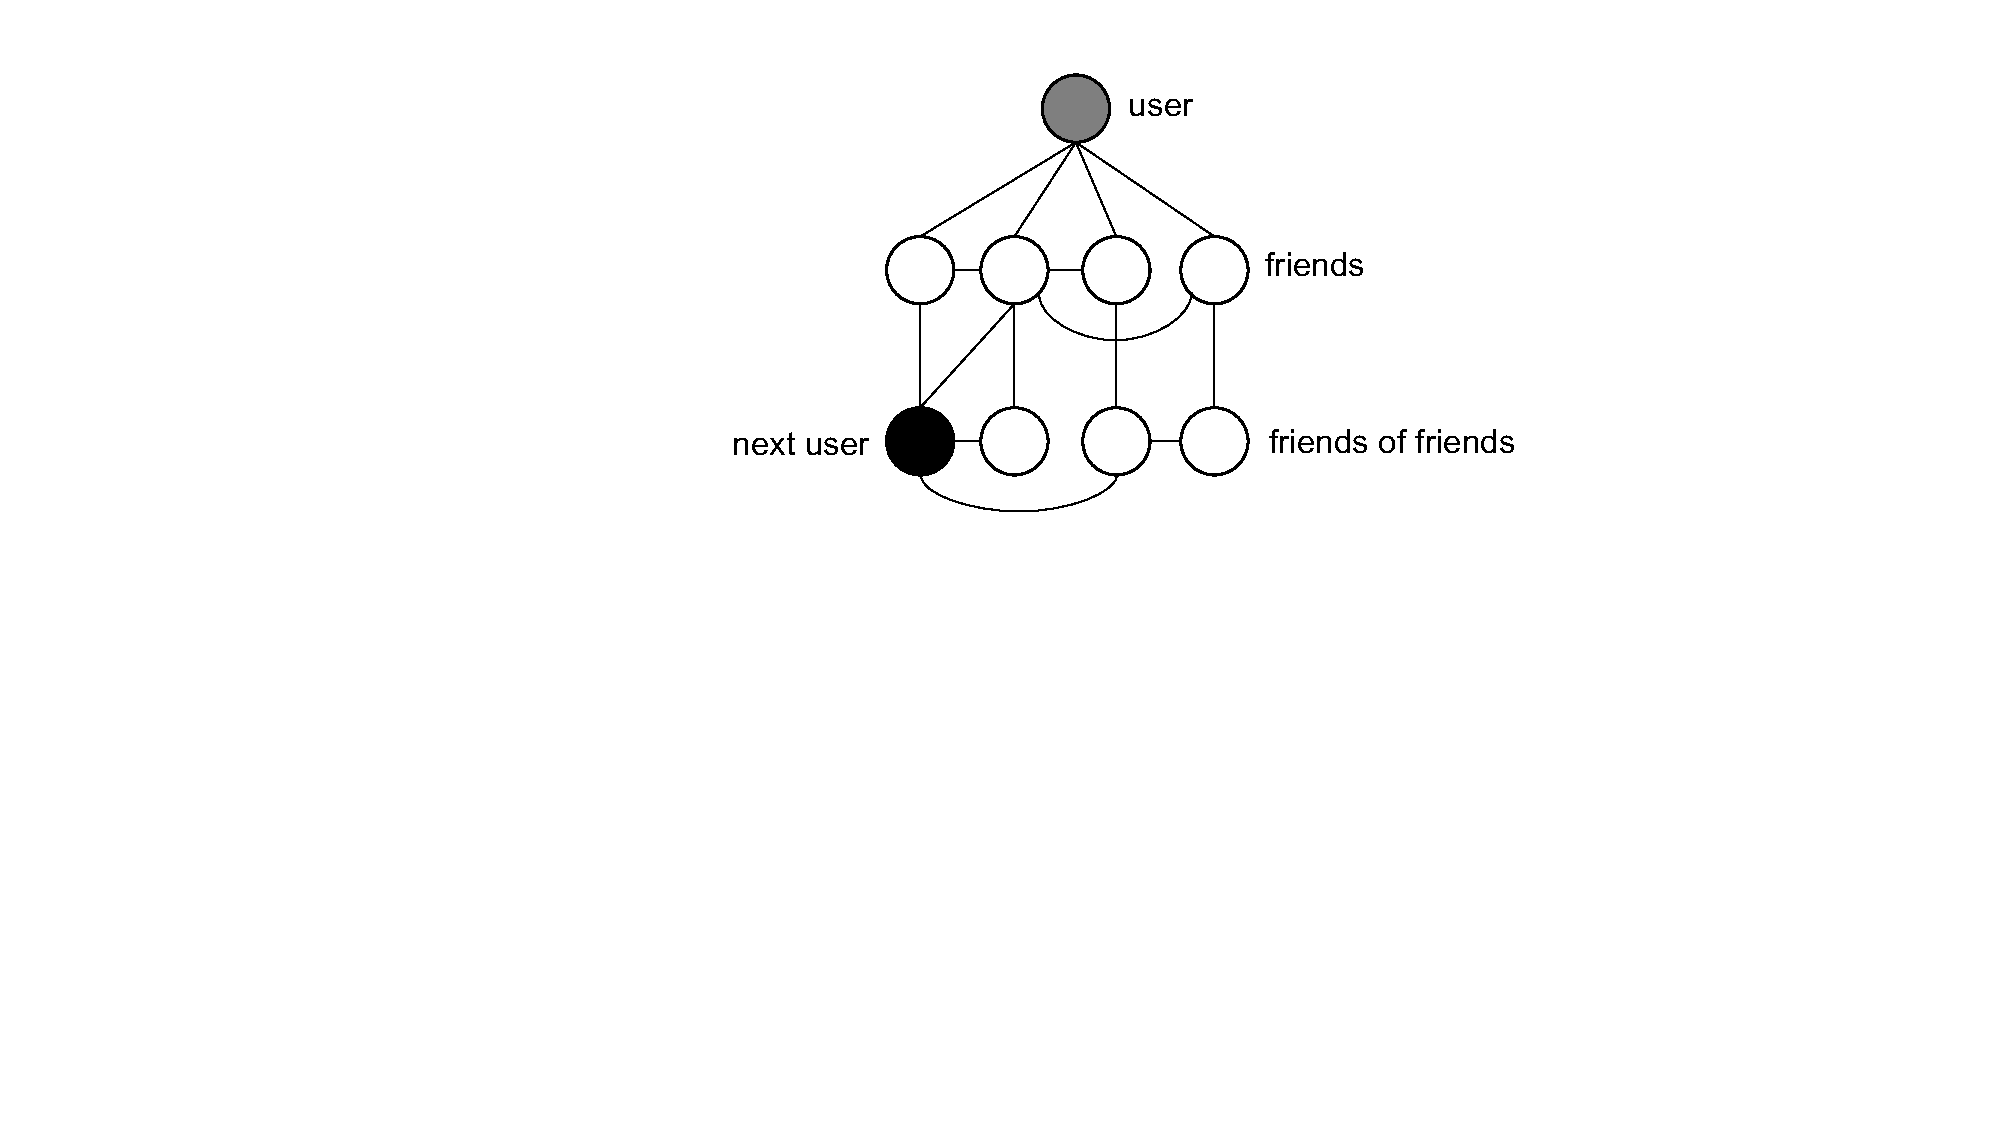
\includegraphics[scale=0.5]{EIB6_graph.pdf}
%An undirected graph representing a triangle: $V=\{1,2,3\}$ and $E=\{(1,2),(1,3),(2,3)\}$
\end{center}
\end{figure}
% ----------
\begin{small}
\begin{verbatim}
foaf(user_1, user_2, d):
  F = friends(user_1) // set user who are friends with user_1
  if user_2 is in F: return d
  FOAF = []
  for f in F:
    if user_2 is in friends(f): return d
    FOAF.append(friends(f) - F) // set subtraction
  max_foaf_count = 0
  max_foaf = NULL
  for f in FOAF:
    foaf_count = | intersect(F,friends(f)) |
    if max_foaf_count < foaf_count:
      max_foaf_count = foaf_count
      max_foaf = f
  foaf(max_foaf, user_2, d+1)
\end{verbatim}
\end{small}
\pagebreak
They seem surprised that, while the algorithm is very fast and give reasonable
results in most cases, every once in a while the algorithm returns a distance
that is different than they expected. Help them understand what assumptions
required for the algorithm they developed and why those are not met here.

\pagebreak

\newpage
\mbox{}
\newpage
\pagebreak
\end{document}
